\begin{frame}{Cell}
    \begin{figure}
        \centering
        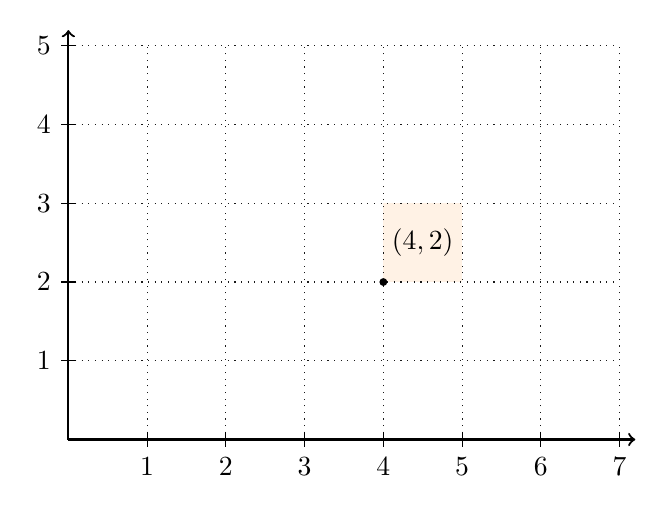
\begin{tikzpicture}
    \fill[orange!10] (4,2) rectangle (5,3);
    \draw[black!90,dotted] (0,0) grid (7,5);
    \draw[thick,->] (0,0) -- (7.2,0);
    \draw[thick,->] (0,0) -- (0,5.2);
    \foreach \x in {1,...,7} {%
        \draw (\x,.1) -- (\x,-.1) node[below] {$\x$};
    }
    \foreach \y in {1,...,5} {%
        \draw (.1,\y) -- (-.1,\y) node[left] {$\y$};
    }
    \fill (4,2) circle (0.05);
    \draw (4.5,2.5) node {$(4,2)$};
\end{tikzpicture}
        \caption{A cell $(c,r)\in\N^2$ defines the region $[c,c+1) \times [r,r+1)$.}
    \end{figure}
\end{frame}

\begin{frame}{Gridded permutation}
    \begin{block}{Definition\hfill(\authcite{albert2012geometric})}
    A pair $(\pi,P)$ where
    \begin{itemize}
        \item $\pi = \pi_1\pi_2 \dotsm \pi_n$ is a permutation
        \item $P = ((c_1,r_1),(c_2,r_2),\dotsc,(c_n,r_n))$ is a $n$-tuple of cells
    \end{itemize}
    is called a \emph{gridded permutation} \onslide<2->{if
    \begin{itemize}
        \item $i<j$ implies $c_i \leq c_j$
        \item $\pi_i < \pi_j$ implies $r_i \leq r_j$
    \end{itemize}
     for all $1 \leq i,j \leq n$.}
    \end{block}
\end{frame}

\begin{frame}{Gridded permutation - example}
\only<1>{\begin{figure}
    \centering
    \begin{tikzpicture}[scale=1.8]
    \draw[opacity=0] (0,0) rectangle (5,3);
    \end{tikzpicture}
    \caption{The gridded permutation with $\pi=87162435$ and $P=((0,2),(0,2),(1,0),(1,2),(1,0),(3,1),(3,0),(4,2))$.}
\end{figure}
\begin{frame}{Cell}
    \begin{figure}
        \centering
        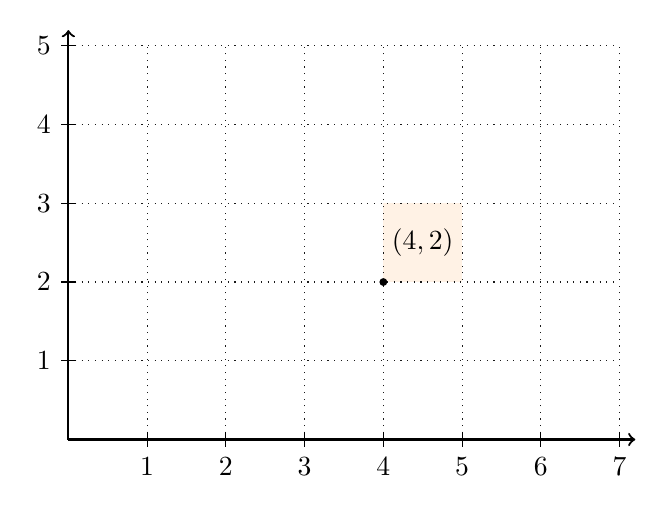
\begin{tikzpicture}
    \fill[orange!10] (4,2) rectangle (5,3);
    \draw[black!90,dotted] (0,0) grid (7,5);
    \draw[thick,->] (0,0) -- (7.2,0);
    \draw[thick,->] (0,0) -- (0,5.2);
    \foreach \x in {1,...,7} {%
        \draw (\x,.1) -- (\x,-.1) node[below] {$\x$};
    }
    \foreach \y in {1,...,5} {%
        \draw (.1,\y) -- (-.1,\y) node[left] {$\y$};
    }
    \fill (4,2) circle (0.05);
    \draw (4.5,2.5) node {$(4,2)$};
\end{tikzpicture}
        \caption{A cell $(c,r)\in\N^2$ defines the region $[c,c+1) \times [r,r+1)$.}
    \end{figure}
\end{frame}

\begin{frame}{Gridded permutation}
    \begin{block}{Definition\hfill(\authcite{albert2012geometric})}
    A pair $(\pi,P)$ where
    \begin{itemize}
        \item $\pi = \pi_1\pi_2 \dotsm \pi_n$ is a permutation
        \item $P = ((c_1,r_1),(c_2,r_2),\dotsc,(c_n,r_n))$ is a $n$-tuple of cells
    \end{itemize}
    is called a \emph{gridded permutation} \onslide<2->{if
    \begin{itemize}
        \item $i<j$ implies $c_i \leq c_j$
        \item $\pi_i < \pi_j$ implies $r_i \leq r_j$
    \end{itemize}
     for all $1 \leq i,j \leq n$.}
    \end{block}
\end{frame}

\begin{frame}{Gridded permutation - example}
\only<1>{\begin{figure}
    \centering
    \begin{tikzpicture}[scale=1.8]
    \draw[opacity=0] (0,0) rectangle (5,3);
    \end{tikzpicture}
    \caption{The gridded permutation with $\pi=87162435$ and $P=((0,2),(0,2),(1,0),(1,2),(1,0),(3,1),(3,0),(4,2))$.}
\end{figure}
\begin{frame}{Cell}
    \begin{figure}
        \centering
        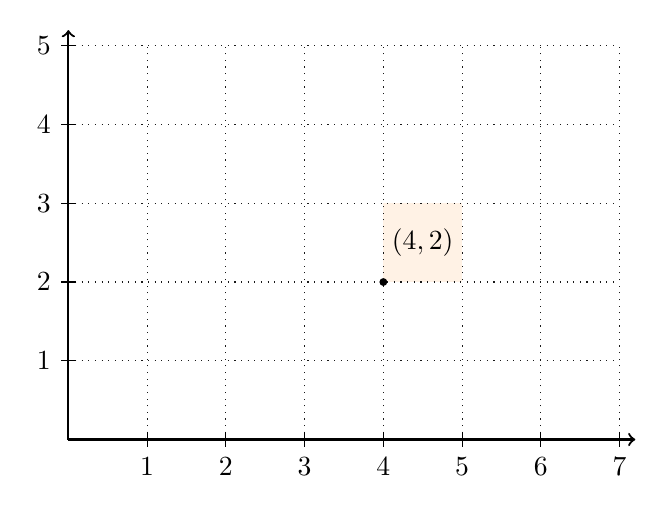
\begin{tikzpicture}
    \fill[orange!10] (4,2) rectangle (5,3);
    \draw[black!90,dotted] (0,0) grid (7,5);
    \draw[thick,->] (0,0) -- (7.2,0);
    \draw[thick,->] (0,0) -- (0,5.2);
    \foreach \x in {1,...,7} {%
        \draw (\x,.1) -- (\x,-.1) node[below] {$\x$};
    }
    \foreach \y in {1,...,5} {%
        \draw (.1,\y) -- (-.1,\y) node[left] {$\y$};
    }
    \fill (4,2) circle (0.05);
    \draw (4.5,2.5) node {$(4,2)$};
\end{tikzpicture}
        \caption{A cell $(c,r)\in\N^2$ defines the region $[c,c+1) \times [r,r+1)$.}
    \end{figure}
\end{frame}

\begin{frame}{Gridded permutation}
    \begin{block}{Definition\hfill(\authcite{albert2012geometric})}
    A pair $(\pi,P)$ where
    \begin{itemize}
        \item $\pi = \pi_1\pi_2 \dotsm \pi_n$ is a permutation
        \item $P = ((c_1,r_1),(c_2,r_2),\dotsc,(c_n,r_n))$ is a $n$-tuple of cells
    \end{itemize}
    is called a \emph{gridded permutation} \onslide<2->{if
    \begin{itemize}
        \item $i<j$ implies $c_i \leq c_j$
        \item $\pi_i < \pi_j$ implies $r_i \leq r_j$
    \end{itemize}
     for all $1 \leq i,j \leq n$.}
    \end{block}
\end{frame}

\begin{frame}{Gridded permutation - example}
\only<1>{\begin{figure}
    \centering
    \begin{tikzpicture}[scale=1.8]
    \draw[opacity=0] (0,0) rectangle (5,3);
    \end{tikzpicture}
    \caption{The gridded permutation with $\pi=87162435$ and $P=((0,2),(0,2),(1,0),(1,2),(1,0),(3,1),(3,0),(4,2))$.}
\end{figure}
\begin{frame}{Cell}
    \begin{figure}
        \centering
        \input{graphics/cell}
        \caption{A cell $(c,r)\in\N^2$ defines the region $[c,c+1) \times [r,r+1)$.}
    \end{figure}
\end{frame}

\begin{frame}{Gridded permutation}
    \begin{block}{Definition\hfill(\authcite{albert2012geometric})}
    A pair $(\pi,P)$ where
    \begin{itemize}
        \item $\pi = \pi_1\pi_2 \dotsm \pi_n$ is a permutation
        \item $P = ((c_1,r_1),(c_2,r_2),\dotsc,(c_n,r_n))$ is a $n$-tuple of cells
    \end{itemize}
    is called a \emph{gridded permutation} \onslide<2->{if
    \begin{itemize}
        \item $i<j$ implies $c_i \leq c_j$
        \item $\pi_i < \pi_j$ implies $r_i \leq r_j$
    \end{itemize}
     for all $1 \leq i,j \leq n$.}
    \end{block}
\end{frame}

\begin{frame}{Gridded permutation - example}
\only<1>{\begin{figure}
    \centering
    \begin{tikzpicture}[scale=1.8]
    \draw[opacity=0] (0,0) rectangle (5,3);
    \end{tikzpicture}
    \caption{The gridded permutation with $\pi=87162435$ and $P=((0,2),(0,2),(1,0),(1,2),(1,0),(3,1),(3,0),(4,2))$.}
\end{figure}
\input{graphics/gp}
}
\addtocounter{figure}{1}
\only<2>{\begin{figure}
    \centering
    \begin{tikzpicture}[scale=1.8]
    \draw[opacity=0] (0,0) rectangle (5,3);
    \end{tikzpicture}
    \caption{An occurrence of $3^{(0,2)}1^{(1,0)}2^{(3,1)}$ in the gridded permutation $87^{(0,2)}1^{(1,0)}6^{(1,2)}2^{(1,0)}4^{(3,1)}3^{(3,0)}5^{(4,2)}$.}
\end{figure}
\input{graphics/gppatt}
}
\end{frame}


%\begin{frame}{Gridded permutation - combinatorial class}
%    \begin{figure}
%        \centering
%        \input{graphics/gpclass}
%        \caption{The combinatorial class $\mathcal{G}^{(5,3)}$.}
%    \end{figure}
%\end{frame}
}
\addtocounter{figure}{1}
\only<2>{\begin{figure}
    \centering
    \begin{tikzpicture}[scale=1.8]
    \draw[opacity=0] (0,0) rectangle (5,3);
    \end{tikzpicture}
    \caption{An occurrence of $3^{(0,2)}1^{(1,0)}2^{(3,1)}$ in the gridded permutation $87^{(0,2)}1^{(1,0)}6^{(1,2)}2^{(1,0)}4^{(3,1)}3^{(3,0)}5^{(4,2)}$.}
\end{figure}
\begin{tikzpicture}[scale=1.8, every node/.style={scale=1.1},overlay,xshift=0.5cm,yshift=1.225cm]
  \def\xs{1.0}
  \def\ys{1.0}
  \def\ps{0.8}
  \draw (0.001,0.001) grid[xscale=\xs,yscale=\ys] (4.999, 2.999);
  \draw[rounded corners=2ex] (0,0) rectangle (5,3);
  \coordinate (p0) at (0.3333333333333333*\xs,2.8*\ys);
  \coordinate (p1) at (0.6666666666666666*\xs,2.6*\ys);
  \coordinate (p2) at (1.25*\xs,0.25*\ys);
  \coordinate (p3) at (1.5*\xs,2.4*\ys);
  \coordinate (p4) at (1.75*\xs,0.5*\ys);
  \coordinate (p5) at (3.3333333333333335*\xs,1.5*\ys);
  \coordinate (p6) at (3.6666666666666665*\xs,0.75*\ys);
  \coordinate (p7) at (4.5*\xs,2.2*\ys);
  \draw (p0)--(p1)--(p2)--(p3)--(p4)--(p5)--(p6)--(p7);
  \fill (p0) circle (0.1*\ps);
  \fill (p1) circle (0.1*\ps);
  \fill (p2) circle (0.1*\ps);
  \fill (p3) circle (0.1*\ps);
  \fill (p4) circle (0.1*\ps);
  \fill (p5) circle (0.1*\ps);
  \fill (p6) circle (0.1*\ps);
  \fill (p7) circle (0.1*\ps);
  \draw[red] (p1) circle (0.15*\ps);
  \draw[red] (p4) circle (0.15*\ps);
  \draw[red] (p5) circle (0.15*\ps);
\end{tikzpicture}
}
\end{frame}


%\begin{frame}{Gridded permutation - combinatorial class}
%    \begin{figure}
%        \centering
%        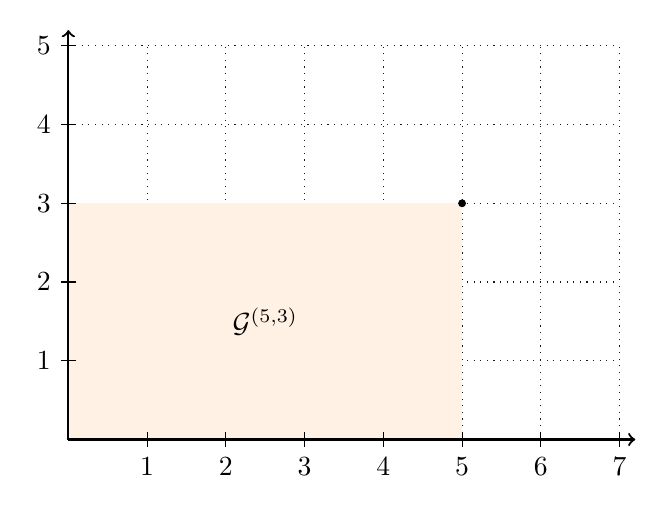
\begin{tikzpicture}
    \draw[black!90,dotted] (0,0) grid (7,5);
    \fill[orange!10] (0,0) rectangle (5,3);
    \draw[thick,->] (0,0) -- (7.2,0);
    \draw[thick,->] (0,0) -- (0,5.2);
    \foreach \x in {1,...,7} {%
        \draw (\x,.1) -- (\x,-.1) node[below] {$\x$};
    }
    \foreach \y in {1,...,5} {%
        \draw (.1,\y) -- (-.1,\y) node[left] {$\y$};
    }
    \fill (5,3) circle (0.05);
    \draw (2.5,1.5) node {$\mathcal{G}^{(5,3)}$};
\end{tikzpicture}
%        \caption{The combinatorial class $\mathcal{G}^{(5,3)}$.}
%    \end{figure}
%\end{frame}
}
\addtocounter{figure}{1}
\only<2>{\begin{figure}
    \centering
    \begin{tikzpicture}[scale=1.8]
    \draw[opacity=0] (0,0) rectangle (5,3);
    \end{tikzpicture}
    \caption{An occurrence of $3^{(0,2)}1^{(1,0)}2^{(3,1)}$ in the gridded permutation $87^{(0,2)}1^{(1,0)}6^{(1,2)}2^{(1,0)}4^{(3,1)}3^{(3,0)}5^{(4,2)}$.}
\end{figure}
\begin{tikzpicture}[scale=1.8, every node/.style={scale=1.1},overlay,xshift=0.5cm,yshift=1.225cm]
  \def\xs{1.0}
  \def\ys{1.0}
  \def\ps{0.8}
  \draw (0.001,0.001) grid[xscale=\xs,yscale=\ys] (4.999, 2.999);
  \draw[rounded corners=2ex] (0,0) rectangle (5,3);
  \coordinate (p0) at (0.3333333333333333*\xs,2.8*\ys);
  \coordinate (p1) at (0.6666666666666666*\xs,2.6*\ys);
  \coordinate (p2) at (1.25*\xs,0.25*\ys);
  \coordinate (p3) at (1.5*\xs,2.4*\ys);
  \coordinate (p4) at (1.75*\xs,0.5*\ys);
  \coordinate (p5) at (3.3333333333333335*\xs,1.5*\ys);
  \coordinate (p6) at (3.6666666666666665*\xs,0.75*\ys);
  \coordinate (p7) at (4.5*\xs,2.2*\ys);
  \draw (p0)--(p1)--(p2)--(p3)--(p4)--(p5)--(p6)--(p7);
  \fill (p0) circle (0.1*\ps);
  \fill (p1) circle (0.1*\ps);
  \fill (p2) circle (0.1*\ps);
  \fill (p3) circle (0.1*\ps);
  \fill (p4) circle (0.1*\ps);
  \fill (p5) circle (0.1*\ps);
  \fill (p6) circle (0.1*\ps);
  \fill (p7) circle (0.1*\ps);
  \draw[red] (p1) circle (0.15*\ps);
  \draw[red] (p4) circle (0.15*\ps);
  \draw[red] (p5) circle (0.15*\ps);
\end{tikzpicture}
}
\end{frame}


%\begin{frame}{Gridded permutation - combinatorial class}
%    \begin{figure}
%        \centering
%        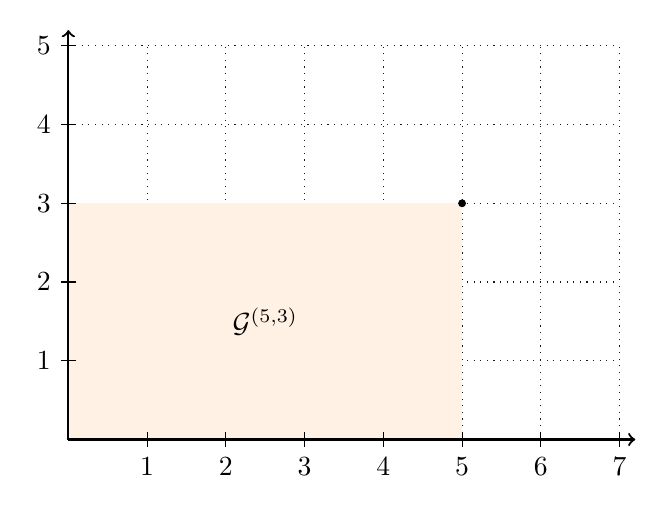
\begin{tikzpicture}
    \draw[black!90,dotted] (0,0) grid (7,5);
    \fill[orange!10] (0,0) rectangle (5,3);
    \draw[thick,->] (0,0) -- (7.2,0);
    \draw[thick,->] (0,0) -- (0,5.2);
    \foreach \x in {1,...,7} {%
        \draw (\x,.1) -- (\x,-.1) node[below] {$\x$};
    }
    \foreach \y in {1,...,5} {%
        \draw (.1,\y) -- (-.1,\y) node[left] {$\y$};
    }
    \fill (5,3) circle (0.05);
    \draw (2.5,1.5) node {$\mathcal{G}^{(5,3)}$};
\end{tikzpicture}
%        \caption{The combinatorial class $\mathcal{G}^{(5,3)}$.}
%    \end{figure}
%\end{frame}
}
\addtocounter{figure}{1}
\only<2>{\begin{figure}
    \centering
    \begin{tikzpicture}[scale=1.8]
    \draw[opacity=0] (0,0) rectangle (5,3);
    \end{tikzpicture}
    \caption{An occurrence of $3^{(0,2)}1^{(1,0)}2^{(3,1)}$ in the gridded permutation $87^{(0,2)}1^{(1,0)}6^{(1,2)}2^{(1,0)}4^{(3,1)}3^{(3,0)}5^{(4,2)}$.}
\end{figure}
\begin{tikzpicture}[scale=1.8, every node/.style={scale=1.1},overlay,xshift=0.5cm,yshift=1.225cm]
  \def\xs{1.0}
  \def\ys{1.0}
  \def\ps{0.8}
  \draw (0.001,0.001) grid[xscale=\xs,yscale=\ys] (4.999, 2.999);
  \draw[rounded corners=2ex] (0,0) rectangle (5,3);
  \coordinate (p0) at (0.3333333333333333*\xs,2.8*\ys);
  \coordinate (p1) at (0.6666666666666666*\xs,2.6*\ys);
  \coordinate (p2) at (1.25*\xs,0.25*\ys);
  \coordinate (p3) at (1.5*\xs,2.4*\ys);
  \coordinate (p4) at (1.75*\xs,0.5*\ys);
  \coordinate (p5) at (3.3333333333333335*\xs,1.5*\ys);
  \coordinate (p6) at (3.6666666666666665*\xs,0.75*\ys);
  \coordinate (p7) at (4.5*\xs,2.2*\ys);
  \draw (p0)--(p1)--(p2)--(p3)--(p4)--(p5)--(p6)--(p7);
  \fill (p0) circle (0.1*\ps);
  \fill (p1) circle (0.1*\ps);
  \fill (p2) circle (0.1*\ps);
  \fill (p3) circle (0.1*\ps);
  \fill (p4) circle (0.1*\ps);
  \fill (p5) circle (0.1*\ps);
  \fill (p6) circle (0.1*\ps);
  \fill (p7) circle (0.1*\ps);
  \draw[red] (p1) circle (0.15*\ps);
  \draw[red] (p4) circle (0.15*\ps);
  \draw[red] (p5) circle (0.15*\ps);
\end{tikzpicture}
}
\end{frame}


%\begin{frame}{Gridded permutation - combinatorial class}
%    \begin{figure}
%        \centering
%        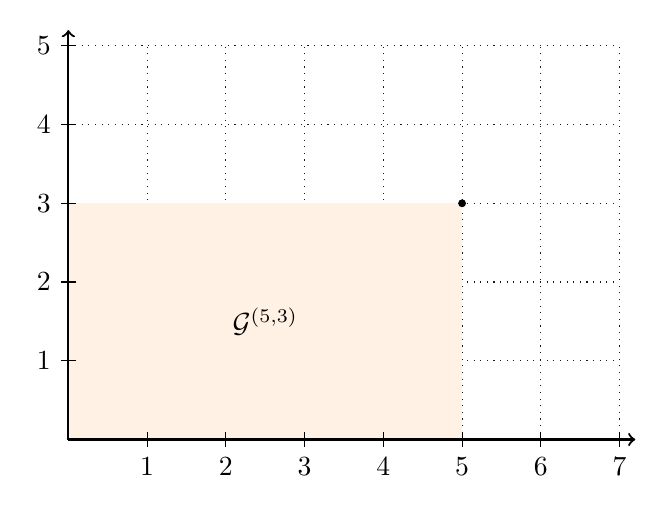
\begin{tikzpicture}
    \draw[black!90,dotted] (0,0) grid (7,5);
    \fill[orange!10] (0,0) rectangle (5,3);
    \draw[thick,->] (0,0) -- (7.2,0);
    \draw[thick,->] (0,0) -- (0,5.2);
    \foreach \x in {1,...,7} {%
        \draw (\x,.1) -- (\x,-.1) node[below] {$\x$};
    }
    \foreach \y in {1,...,5} {%
        \draw (.1,\y) -- (-.1,\y) node[left] {$\y$};
    }
    \fill (5,3) circle (0.05);
    \draw (2.5,1.5) node {$\mathcal{G}^{(5,3)}$};
\end{tikzpicture}
%        \caption{The combinatorial class $\mathcal{G}^{(5,3)}$.}
%    \end{figure}
%\end{frame}